% ============================================================
%  SLIDE GALLERY — 幻灯片样例库
%  本文件收录常用 Beamer 幻灯片布局和 LaTeX 构件，供复制参考。
%  在 main.tex 的 \appendix 块内加入：
%      % ============================================================
%  SLIDE GALLERY — 幻灯片样例库
%  本文件收录常用 Beamer 幻灯片布局和 LaTeX 构件，供复制参考。
%  在 main.tex 的 \appendix 块内加入：
%      % ============================================================
%  SLIDE GALLERY — 幻灯片样例库
%  本文件收录常用 Beamer 幻灯片布局和 LaTeX 构件，供复制参考。
%  在 main.tex 的 \appendix 块内加入：
%      % ============================================================
%  SLIDE GALLERY — 幻灯片样例库
%  本文件收录常用 Beamer 幻灯片布局和 LaTeX 构件，供复制参考。
%  在 main.tex 的 \appendix 块内加入：
%      \input{sections/00_slide_gallery}
%  即可将本库编译进文档。
% ============================================================

\section{Slide Gallery}

% ------------------------------------------------------------------
\subsection{文字与列表 / Text \& Lists}
% ------------------------------------------------------------------

\begin{frame}{Itemize — 三级嵌套}
  \begin{itemize}
    \item 一级条目（默认样式）
      \begin{itemize}
        \item 二级条目（缩进更深）
          \begin{itemize}
            \item 三级条目（通常避免超过三级）
          \end{itemize}
      \end{itemize}
    \item 另一条一级条目
    \item 再一条一级条目
  \end{itemize}
\end{frame}

\begin{frame}{Enumerate — 有序列表}
  \begin{enumerate}
    \item 第一步：提出问题
    \item 第二步：建立模型
      \begin{enumerate}
        \item 子步骤 A
        \item 子步骤 B
      \end{enumerate}
    \item 第三步：实证检验
    \item 第四步：政策含义
  \end{enumerate}
\end{frame}

\begin{frame}{Description — 术语表}
  \begin{description}
    \item[识别 (Identification)] 将因果效应与相关性分离的策略。
    \item[工具变量 (IV)] 影响处理变量但不直接影响结果的变量。
    \item[排除限制 (Exclusion)] 工具变量仅通过处理变量影响结果。
    \item[外生性 (Exogeneity)] 工具变量与误差项不相关的假设。
  \end{description}
\end{frame}

\begin{frame}{强调与颜色}
  \begin{itemize}
    \item 使用 \alert{alert} 将关键词标红（beamer 默认强调色）。
    \item 使用 \textbf{粗体}表示重要概念。
    \item 使用 \textit{斜体}表示书名、外文词汇。
    \item 使用 \textcolor{blue}{自定义颜色}：\texttt{\textbackslash textcolor\{blue\}\{...\}}。
    \item 使用 \colorbox{yellow!40}{背景高亮}：\texttt{\textbackslash colorbox\{yellow!40\}\{...\}}。
    \item \structure{结构色}（beamer \texttt{\textbackslash structure}）跟随主题变化。
  \end{itemize}
\end{frame}

% ------------------------------------------------------------------
\subsection{分栏布局 / Column Layouts}
% ------------------------------------------------------------------

\begin{frame}{两栏均等 50/50}
  \begin{columns}[T]
    \column{0.5\textwidth}
      \textbf{左栏}
      \begin{itemize}
        \item 论点一
        \item 论点二
        \item 论点三
      \end{itemize}
    \column{0.5\textwidth}
      \textbf{右栏}
      \begin{itemize}
        \item 反驳一
        \item 反驳二
        \item 反驳三
      \end{itemize}
  \end{columns}
\end{frame}

\begin{frame}{两栏不等 60/40（文字 + 图）}
  \begin{columns}[T]
    \column{0.60\textwidth}
      \begin{itemize}
        \item 宽栏放主要论述，窄栏放配图或摘要。
        \item 保持每条 bullet 简短，避免折行过多。
        \item 此布局适合"文字驱动"幻灯片。
      \end{itemize}
    \column{0.40\textwidth}
      \centering
      
\includegraphics[width=\linewidth]{figures/example-diagram.pdf}
      \par\smallskip
      {\tiny 图注：替换为实际图形。}
  \end{columns}
\end{frame}

\begin{frame}{三栏等宽}
  \begin{columns}[T]
    \column{0.33\textwidth}
      \centering
      \textbf{阶段一}\\[6pt]
      描述第一阶段的核心特征或数据。
    \column{0.33\textwidth}
      \centering
      \textbf{阶段二}\\[6pt]
      描述第二阶段的核心特征或数据。
    \column{0.34\textwidth}
      \centering
      \textbf{阶段三}\\[6pt]
      描述第三阶段的核心特征或数据。
  \end{columns}
\end{frame}

% ------------------------------------------------------------------
\subsection{块与定理 / Blocks \& Theorems}
% ------------------------------------------------------------------

\begin{frame}{三种标准块}
  \begin{block}{标准块 (block)}
    用于关键事实、定义、或中性信息。
  \end{block}
  \begin{alertblock}{警示块 (alertblock)}
    用于警告、重要假设、或关键局限性。
  \end{alertblock}
  \begin{exampleblock}{示例块 (exampleblock)}
    用于数值例子、实证事实、或直觉说明。
  \end{exampleblock}
\end{frame}

\begin{frame}{定理与推论}
  \begin{theorem}[包络定理]
    设 $V(\theta) = \max_x f(x, \theta)$，则
    $\dfrac{dV}{d\theta} = \dfrac{\partial f}{\partial \theta}\big|_{x=x^*(\theta)}$。
  \end{theorem}
  \begin{corollary}
    在可微条件下，值函数关于参数的单调性由 $\partial f/\partial\theta$ 的符号决定。
  \end{corollary}
\end{frame}

\begin{frame}{定义与引理}
  \begin{definition}[纳什均衡]
    策略组合 $\sigma^*$ 是纳什均衡，当且仅当对任意参与人 $i$，
    在其他人策略不变的情况下，$i$ 无法通过单边偏离获益。
  \end{definition}
  \begin{lemma}
    任何有限博弈在混合策略意义下至少存在一个纳什均衡。
  \end{lemma}
\end{frame}

\begin{frame}{证明框架}
  \begin{proof}
    设 $x^* \notin \arg\max f(x)$，则存在 $x'$ 使得 $f(x') > f(x^*)$，
    与 $x^*$ 的最优性矛盾。故 $x^*$ 确为最大值点。
  \end{proof}
  \medskip
  \begin{exampleblock}{规范说明}
    Beamer 自动在 proof 结尾添加 $\square$，无需手动输入。
  \end{exampleblock}
\end{frame}

% ------------------------------------------------------------------
\subsection{数学公式 / Math}
% ------------------------------------------------------------------

\begin{frame}{行内与独行公式}
  行内公式：$\hat{\beta} = (X^\top X)^{-1} X^\top y$，
  或 $\text{plim}\,\hat{\beta} = \beta + (X^\top X/n)^{-1}(X^\top \varepsilon/n)$。

  \[
    \sigma^2 = \frac{1}{n}\sum_{i=1}^{n}(x_i - \bar{x})^2, \qquad
    \bar{x} = \frac{1}{n}\sum_{i=1}^{n} x_i.
  \]
\end{frame}

\begin{frame}{Align 带编号}
  \begin{align}
    \ell(\beta) &= \sum_{i=1}^{n}
      \bigl[y_i \log p_i + (1-y_i)\log(1-p_i)\bigr], \label{eq:loglik} \\
    \frac{\partial \ell}{\partial \beta} &= X^\top(y - p) = 0. \label{eq:foc}
  \end{align}
  式 \eqref{eq:loglik} 为对数似然；式 \eqref{eq:foc} 为一阶条件。
\end{frame}

\begin{frame}{矩阵}
  \[
    A = \begin{pmatrix} a_{11} & a_{12} \\ a_{21} & a_{22} \end{pmatrix}, \qquad
    B = \begin{bmatrix} 1 & 0 & 0 \\ 0 & 1 & 0 \\ 0 & 0 & 1 \end{bmatrix}, \qquad
    \det(A) = a_{11}a_{22} - a_{12}a_{21}.
  \]
\end{frame}

\begin{frame}{分段函数与 Cases}
  \[
    f(x) = \begin{cases}
      \alpha + \beta x   & \text{若 } x \geq \bar{x}, \\[4pt]
      \gamma + \delta x  & \text{若 } x < \bar{x}.
    \end{cases}
  \]
  \medskip
  注：用 \texttt{\\[4pt]} 在 cases 各行之间增加垂直间距。
\end{frame}

\begin{frame}{优化问题}
  \[
    \max_{\{c_t,\,k_{t+1}\}_{t=0}^{\infty}}
    \sum_{t=0}^{\infty} \beta^t u(c_t)
  \]
  \[
    \text{s.t.} \quad c_t + k_{t+1} = A k_t^\alpha, \quad
    c_t \geq 0, \quad k_0 \text{ 给定}.
  \]
  \begin{itemize}
    \item $\beta \in (0,1)$：折现因子；\quad $\alpha \in (0,1)$：资本份额。
    \item 贝尔曼方程：$V(k) = \max_{k'} \bigl\{u(Ak^\alpha - k') + \beta V(k')\bigr\}$。
  \end{itemize}
\end{frame}

% ------------------------------------------------------------------
\subsection{叠加动画 / Overlays \& Animations}
% ------------------------------------------------------------------

\begin{frame}{逐步显示：\texttt{\textbackslash pause}}
  \begin{itemize}
    \item 第一条：出现在第 1 页。
    \pause
    \item 第二条：出现在第 2 页。
    \pause
    \item 第三条：出现在第 3 页。
  \end{itemize}
  \pause
  \begin{exampleblock}{小结（第 4 页）}
    结合具体内容决定在何处插入 \texttt{\textbackslash pause}。
  \end{exampleblock}
\end{frame}

\begin{frame}{条件替换：\texttt{\textbackslash only}}
  \only<1>{
    \begin{block}{步骤 1 — 建模}
      定义参与人、策略空间和支付函数。
    \end{block}
  }
  \only<2>{
    \begin{block}{步骤 2 — 求解}
      对每位参与人求最优反应函数，联立求解。
    \end{block}
  }
  \only<3>{
    \begin{block}{步骤 3 — 解读}
      分析均衡的经济含义与福利性质。
    \end{block}
  }
  \vspace{0.5cm}
  \centering\footnotesize
  [\only<1>{第 1/3 页}\only<2>{第 2/3 页}\only<3>{第 3/3 页}]
\end{frame}

\begin{frame}{关键词逐步高亮：\texttt{\textbackslash alert<>}}
  估计策略分三步：
  \begin{itemize}
    \item<1-> \alert<1>{识别}：利用准随机变异剥离内生性。
    \item<2-> \alert<2>{估计}：对简约式做 OLS，获得降维方程。
    \item<3-> \alert<3>{推断}：使用聚类稳健标准误进行显著性检验。
  \end{itemize}
\end{frame}

\begin{frame}{未来条目置灰：\texttt{transparent}}
  {%  使用大括号将效果限制在本帧
    \setbeamercovered{transparent}
    \begin{itemize}
      \item<1-> 条目一（第 1 页完全可见，后续置灰）
      \item<2-> 条目二（第 2 页完全可见）
      \item<3-> 条目三（第 3 页完全可见）
    \end{itemize}
  }
\end{frame}

% ------------------------------------------------------------------
\subsection{图形与 TikZ / Figures \& TikZ}
% ------------------------------------------------------------------

\begin{frame}{并排双图（minipage）}
  \begin{columns}[c]
    \column{0.48\textwidth}
      \begin{figure}
        \centering
        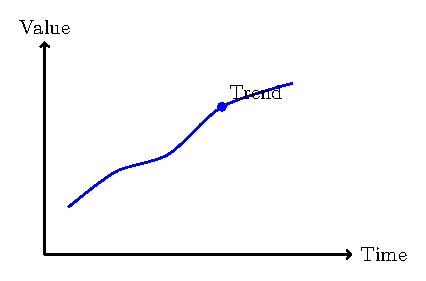
\includegraphics[width=\linewidth,height=0.48\textheight,
                         keepaspectratio]{figures/example-chart.pdf}
        \caption{面板 A：处理组}
      \end{figure}
    \column{0.48\textwidth}
      \begin{figure}
        \centering
        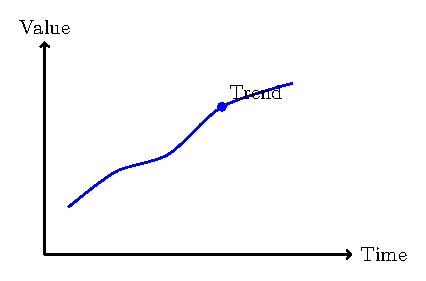
\includegraphics[width=\linewidth,height=0.48\textheight,
                         keepaspectratio]{figures/example-chart.pdf}
        \caption{面板 B：对照组}
      \end{figure}
  \end{columns}
\end{frame}

\begin{frame}{TikZ — 因果有向图 (DAG)}
  \centering
  \begin{tikzpicture}[
      node distance=1.8cm and 2.6cm,
      box/.style={draw, rounded corners=4pt,
                  minimum width=1.9cm, minimum height=0.65cm,
                  font=\small, fill=white},
      >=Stealth, thick
    ]
    \node[box] (Z) {工具变量 $Z$};
    \node[box, right=of Z] (X) {处理变量 $X$};
    \node[box, right=of X] (Y) {结果变量 $Y$};
    \node[box, dashed, above right=0.55cm and 0.9cm of X]
          (U) {不可观测 $U$};
    \draw[->] (Z) -- (X);
    \draw[->] (X) -- (Y);
    \draw[->, dashed, gray] (U) -- (X);
    \draw[->, dashed, gray] (U) -- (Y);
    \draw[->, red!70!black, bend right=18]
          node[below, font=\scriptsize, midway]{排除限制} (Z.south) to (Y.south);
    % 注：上面的 bend right 箭头演示"违反排除限制"的情形，
    %     实际使用时可删去。
  \end{tikzpicture}
  \par\smallskip
  {\footnotesize 虚线 = 不可观测路径；红色弯箭头 = 违反排除限制（示意）。}
\end{frame}

\begin{frame}{TikZ — 流程图}
  \centering
  \begin{tikzpicture}[
      node distance=0.75cm,
      box/.style={draw, rounded corners=3pt,
                  minimum width=3.4cm, minimum height=0.58cm,
                  align=center, font=\small, fill=blue!5},
      dec/.style={draw, diamond, aspect=2.6,
                  minimum width=2.8cm, font=\small, fill=orange!10},
      >=Stealth, thick
    ]
    \node[box]  (data)  {原始数据};
    \node[box, below=of data]  (clean) {清洗与预处理};
    \node[dec, below=of clean] (valid) {通过质检？};
    \node[box, below=of valid] (est)   {模型估计};
    \node[box, below=of est]   (rep)   {报告结果};

    \draw[->] (data)  -- (clean);
    \draw[->] (clean) -- (valid);
    \draw[->] (valid) -- node[right, font=\scriptsize]{是} (est);
    \draw[->] (valid.west) -- ++(-1.3,0)
              |- node[left, font=\scriptsize, pos=0.22]{否} (clean.west);
    \draw[->] (est)   -- (rep);
  \end{tikzpicture}
\end{frame}
\begin{frame}{TikZ — 水平时间轴}
  \centering
  \begin{tikzpicture}[>=Stealth, thick, font=\small]
    
    % 1. 调整背景框的深度（下移至 -0.85）
    \fill[blue!15, rounded corners=2pt] (2.2,-0.55) rectangle (6.8, 0.05);
    % 2. 将“样本期间”文字下移（Y坐标从 -0.35 改为 -0.65），避开“2008”
    \node[font=\scriptsize, text=blue!60!black] at (4.5,-0.65) {样本期间};

    % 3. 绘制主时间轴和年份刻度
    \draw[->] (-0.3,0) -- (9.2,0) node[right] {年份};
    \foreach \x/\yr in {0.5/1990, 2.5/2000, 4.5/2008, 6.5/2015, 8.5/2023}{
      \draw (\x, 0.12) -- (\x,-0.12) node[below] {\yr};
    }
    
    % 4. 事件标注（上方）
    \node[above, align=center, font=\scriptsize] at (0.5, 0.22) {改革 A};
    \node[above, align=center, font=\scriptsize] at (2.5, 0.22) {改革 B};
    \node[above, align=center, font=\scriptsize, text=red!70!black]
          at (4.5, 0.22) {金融危机};
    \node[above, align=center, font=\scriptsize] at (6.5, 0.22) {政策 C};
    \node[above, align=center, font=\scriptsize] at (8.5, 0.22) {今日};
    
    % 5. 当前位置标记
    \draw[red!70!black, thick] (8.5,0.35) -- (8.5,-0.12);
    
  \end{tikzpicture}
\end{frame}
% ------------------------------------------------------------------
\subsection{表格样例 / Tables}
% ------------------------------------------------------------------

\begin{frame}{描述性统计}
  \input{tables/summary-stats}
\end{frame}

\begin{frame}{多列回归比较}
  \input{tables/reg-comparison}
\end{frame}

\begin{frame}[shrink=20]{双面板（Panel A / B）异质性}
  \input{tables/twopart-table}
\end{frame}

\begin{frame}{行高亮表格（colortbl）}
  % 需要在 main.tex 中加载 \usepackage{colortbl}
  \begin{table}
    \centering
    \caption{带高亮行的表格示例}
    \begin{tabular}{lcc}
      \toprule
      变量 & 处理组 & 对照组 \\
      \midrule
      \rowcolor{yellow!30}
      GDP 增速 (\%) & 6.8 & 3.2 \\
      失业率 (\%)   & 4.1 & 7.6 \\
      \rowcolor{yellow!30}
      通货膨胀 (\%) & 2.3 & 4.8 \\
      贸易开放度    & 0.72 & 0.51 \\
      \bottomrule
    \end{tabular}
  \end{table}
  {\footnotesize \textit{注}：黄色行为核心关注变量。}
\end{frame}

% ------------------------------------------------------------------
\subsection{代码与逐字排版 / Code \& Verbatim}
% ------------------------------------------------------------------

\begin{frame}[fragile]{Python 代码（listings）}
  % 需要在 main.tex 中加载 \usepackage{listings} 并配置 \lstset
  \begin{lstlisting}[language=Python, caption={OLS 估计量（NumPy 实现）}]
import numpy as np

def ols(X, y):
    """返回 OLS 系数向量 beta_hat."""
    return np.linalg.solve(X.T @ X, X.T @ y)

# 生成模拟数据
rng  = np.random.default_rng(42)
X    = np.column_stack([np.ones(200), rng.standard_normal((200, 2))])
beta = np.array([1.0, 2.0, -0.5])
y    = X @ beta + rng.standard_normal(200)

print(ols(X, y))   # 应接近 [1, 2, -0.5]
  \end{lstlisting}
\end{frame}

\begin{frame}[fragile]{LaTeX 代码排版（lstlisting）}
  % ⚠ Beamer 限制：[fragile] 帧的内容（含 \input 子文件）里
  %   不能出现字面的 \end{frame}，否则 Beamer 预扫描会误判帧结束。
  %   解决方法：只展示帧内部代码，外层 \begin/\end{frame} 用文字说明。
  \begin{lstlisting}[language=TeX, caption={帧内叠加动画（内部代码）}]
% 以下内容放在 frame 环境内部（外层为 \begin{frame}...\end{...} 结构）：
\begin{itemize}
  \item<1-> \alert<1>{Step 1}: 建立模型
  \item<2-> \alert<2>{Step 2}: 求解均衡
  \item<3-> \alert<3>{Step 3}: 实证检验
\end{itemize}
\setbeamercovered{transparent}  % 未到场条目置灰
  \end{lstlisting}
  {\footnotesize\textit{注}：若需在代码块中展示完整帧结构（含 \texttt{\textbackslash end\{frame\}}），
  可将代码存入独立 \texttt{.tex} 文件后用 \texttt{\textbackslash lstinputlisting} 引入。}
\end{frame}

% ------------------------------------------------------------------
\subsection{特殊幻灯片与导航 / Special Slides \& Navigation}
% ------------------------------------------------------------------

\begin{frame}{章节过渡页}
  \vspace*{\fill}
  \begin{center}
    {\Large \textbf{第~\Roman{section}~部分}}\\[0.7em]
    {\large \insertsectionhead}\\[1.2em]
    {\normalsize 一句话预告本节核心内容。}
  \end{center}
  \vspace*{\fill}
\end{frame}

\begin{frame}{进度路线图（手动高亮当前节）}
  \begin{enumerate}
    \item[\checkmark] 引言
    \item[\checkmark] 背景与文献
    \item[\textbf{3.}] \textbf{模型} \quad \textcolor{blue}{$\leftarrow$ 当前}
    \item[4.] \textcolor{gray}{实证分析}
    \item[5.] \textcolor{gray}{结论}
  \end{enumerate}
\end{frame}

\begin{frame}{两箱对比（alertblock vs exampleblock）}
  \begin{columns}[T]
    \column{0.48\textwidth}
      \begin{alertblock}{无干预（基准）}
        \begin{itemize}
          \item 产出增速：低
          \item 失业率：高
          \item 社会福利：$W_0$
        \end{itemize}
      \end{alertblock}
    \column{0.48\textwidth}
      \begin{exampleblock}{有干预（反事实）}
        \begin{itemize}
          \item 产出增速：高
          \item 失业率：低
          \item 社会福利：$W_1 > W_0$
        \end{itemize}
      \end{exampleblock}
  \end{columns}
\end{frame}

\begin{frame}{引言页 / Pull Quote}
  \vspace*{\fill}
  \begin{center}
    \Large\itshape
    ``好的模型不求包罗万象，\\
    只求能对关键机制给出清晰预测。''
    \vspace{0.9em}

    \normalsize\upshape
    --- 示例引用，\textit{来源书目}，年份
  \end{center}
  \vspace*{\fill}
\end{frame}

% 超链接导航示例
% 用法：目标帧内加 \label{frm:target}，此处用 \hyperlink{frm:target}{按钮}
\begin{frame}{附录跳转按钮}
  正文幻灯片可加入指向附录的按钮，听众提问时快速跳转：

  \medskip
  \hyperlink{frm:robustness}{\beamergotobutton{稳健性检验}}
  \hspace{1em}
  \hyperlink{frm:derivation}{\beamergotobutton{完整推导}}
  \hspace{1em}
  \hyperlink{frm:data}{\beamergotobutton{数据说明}}

  \bigskip
  附录帧返回正文：

  \medskip
  \hyperlink{frm:main-results}{\beamerreturnbutton{返回主结果}}
  \hspace{1em}
  \hyperlink{frm:empirics}{\beamerbutton{跳至实证节}}

  \bigskip
  {\footnotesize \textit{用法}：在目标帧内加
    \texttt{\textbackslash label\{frm:robustness\}} 等标签即可激活以上按钮。}
\end{frame}

%  即可将本库编译进文档。
% ============================================================

\section{Slide Gallery}

% ------------------------------------------------------------------
\subsection{文字与列表 / Text \& Lists}
% ------------------------------------------------------------------

\begin{frame}{Itemize — 三级嵌套}
  \begin{itemize}
    \item 一级条目（默认样式）
      \begin{itemize}
        \item 二级条目（缩进更深）
          \begin{itemize}
            \item 三级条目（通常避免超过三级）
          \end{itemize}
      \end{itemize}
    \item 另一条一级条目
    \item 再一条一级条目
  \end{itemize}
\end{frame}

\begin{frame}{Enumerate — 有序列表}
  \begin{enumerate}
    \item 第一步：提出问题
    \item 第二步：建立模型
      \begin{enumerate}
        \item 子步骤 A
        \item 子步骤 B
      \end{enumerate}
    \item 第三步：实证检验
    \item 第四步：政策含义
  \end{enumerate}
\end{frame}

\begin{frame}{Description — 术语表}
  \begin{description}
    \item[识别 (Identification)] 将因果效应与相关性分离的策略。
    \item[工具变量 (IV)] 影响处理变量但不直接影响结果的变量。
    \item[排除限制 (Exclusion)] 工具变量仅通过处理变量影响结果。
    \item[外生性 (Exogeneity)] 工具变量与误差项不相关的假设。
  \end{description}
\end{frame}

\begin{frame}{强调与颜色}
  \begin{itemize}
    \item 使用 \alert{alert} 将关键词标红（beamer 默认强调色）。
    \item 使用 \textbf{粗体}表示重要概念。
    \item 使用 \textit{斜体}表示书名、外文词汇。
    \item 使用 \textcolor{blue}{自定义颜色}：\texttt{\textbackslash textcolor\{blue\}\{...\}}。
    \item 使用 \colorbox{yellow!40}{背景高亮}：\texttt{\textbackslash colorbox\{yellow!40\}\{...\}}。
    \item \structure{结构色}（beamer \texttt{\textbackslash structure}）跟随主题变化。
  \end{itemize}
\end{frame}

% ------------------------------------------------------------------
\subsection{分栏布局 / Column Layouts}
% ------------------------------------------------------------------

\begin{frame}{两栏均等 50/50}
  \begin{columns}[T]
    \column{0.5\textwidth}
      \textbf{左栏}
      \begin{itemize}
        \item 论点一
        \item 论点二
        \item 论点三
      \end{itemize}
    \column{0.5\textwidth}
      \textbf{右栏}
      \begin{itemize}
        \item 反驳一
        \item 反驳二
        \item 反驳三
      \end{itemize}
  \end{columns}
\end{frame}

\begin{frame}{两栏不等 60/40（文字 + 图）}
  \begin{columns}[T]
    \column{0.60\textwidth}
      \begin{itemize}
        \item 宽栏放主要论述，窄栏放配图或摘要。
        \item 保持每条 bullet 简短，避免折行过多。
        \item 此布局适合"文字驱动"幻灯片。
      \end{itemize}
    \column{0.40\textwidth}
      \centering
      
\includegraphics[width=\linewidth]{figures/example-diagram.pdf}
      \par\smallskip
      {\tiny 图注：替换为实际图形。}
  \end{columns}
\end{frame}

\begin{frame}{三栏等宽}
  \begin{columns}[T]
    \column{0.33\textwidth}
      \centering
      \textbf{阶段一}\\[6pt]
      描述第一阶段的核心特征或数据。
    \column{0.33\textwidth}
      \centering
      \textbf{阶段二}\\[6pt]
      描述第二阶段的核心特征或数据。
    \column{0.34\textwidth}
      \centering
      \textbf{阶段三}\\[6pt]
      描述第三阶段的核心特征或数据。
  \end{columns}
\end{frame}

% ------------------------------------------------------------------
\subsection{块与定理 / Blocks \& Theorems}
% ------------------------------------------------------------------

\begin{frame}{三种标准块}
  \begin{block}{标准块 (block)}
    用于关键事实、定义、或中性信息。
  \end{block}
  \begin{alertblock}{警示块 (alertblock)}
    用于警告、重要假设、或关键局限性。
  \end{alertblock}
  \begin{exampleblock}{示例块 (exampleblock)}
    用于数值例子、实证事实、或直觉说明。
  \end{exampleblock}
\end{frame}

\begin{frame}{定理与推论}
  \begin{theorem}[包络定理]
    设 $V(\theta) = \max_x f(x, \theta)$，则
    $\dfrac{dV}{d\theta} = \dfrac{\partial f}{\partial \theta}\big|_{x=x^*(\theta)}$。
  \end{theorem}
  \begin{corollary}
    在可微条件下，值函数关于参数的单调性由 $\partial f/\partial\theta$ 的符号决定。
  \end{corollary}
\end{frame}

\begin{frame}{定义与引理}
  \begin{definition}[纳什均衡]
    策略组合 $\sigma^*$ 是纳什均衡，当且仅当对任意参与人 $i$，
    在其他人策略不变的情况下，$i$ 无法通过单边偏离获益。
  \end{definition}
  \begin{lemma}
    任何有限博弈在混合策略意义下至少存在一个纳什均衡。
  \end{lemma}
\end{frame}

\begin{frame}{证明框架}
  \begin{proof}
    设 $x^* \notin \arg\max f(x)$，则存在 $x'$ 使得 $f(x') > f(x^*)$，
    与 $x^*$ 的最优性矛盾。故 $x^*$ 确为最大值点。
  \end{proof}
  \medskip
  \begin{exampleblock}{规范说明}
    Beamer 自动在 proof 结尾添加 $\square$，无需手动输入。
  \end{exampleblock}
\end{frame}

% ------------------------------------------------------------------
\subsection{数学公式 / Math}
% ------------------------------------------------------------------

\begin{frame}{行内与独行公式}
  行内公式：$\hat{\beta} = (X^\top X)^{-1} X^\top y$，
  或 $\text{plim}\,\hat{\beta} = \beta + (X^\top X/n)^{-1}(X^\top \varepsilon/n)$。

  \[
    \sigma^2 = \frac{1}{n}\sum_{i=1}^{n}(x_i - \bar{x})^2, \qquad
    \bar{x} = \frac{1}{n}\sum_{i=1}^{n} x_i.
  \]
\end{frame}

\begin{frame}{Align 带编号}
  \begin{align}
    \ell(\beta) &= \sum_{i=1}^{n}
      \bigl[y_i \log p_i + (1-y_i)\log(1-p_i)\bigr], \label{eq:loglik} \\
    \frac{\partial \ell}{\partial \beta} &= X^\top(y - p) = 0. \label{eq:foc}
  \end{align}
  式 \eqref{eq:loglik} 为对数似然；式 \eqref{eq:foc} 为一阶条件。
\end{frame}

\begin{frame}{矩阵}
  \[
    A = \begin{pmatrix} a_{11} & a_{12} \\ a_{21} & a_{22} \end{pmatrix}, \qquad
    B = \begin{bmatrix} 1 & 0 & 0 \\ 0 & 1 & 0 \\ 0 & 0 & 1 \end{bmatrix}, \qquad
    \det(A) = a_{11}a_{22} - a_{12}a_{21}.
  \]
\end{frame}

\begin{frame}{分段函数与 Cases}
  \[
    f(x) = \begin{cases}
      \alpha + \beta x   & \text{若 } x \geq \bar{x}, \\[4pt]
      \gamma + \delta x  & \text{若 } x < \bar{x}.
    \end{cases}
  \]
  \medskip
  注：用 \texttt{\\[4pt]} 在 cases 各行之间增加垂直间距。
\end{frame}

\begin{frame}{优化问题}
  \[
    \max_{\{c_t,\,k_{t+1}\}_{t=0}^{\infty}}
    \sum_{t=0}^{\infty} \beta^t u(c_t)
  \]
  \[
    \text{s.t.} \quad c_t + k_{t+1} = A k_t^\alpha, \quad
    c_t \geq 0, \quad k_0 \text{ 给定}.
  \]
  \begin{itemize}
    \item $\beta \in (0,1)$：折现因子；\quad $\alpha \in (0,1)$：资本份额。
    \item 贝尔曼方程：$V(k) = \max_{k'} \bigl\{u(Ak^\alpha - k') + \beta V(k')\bigr\}$。
  \end{itemize}
\end{frame}

% ------------------------------------------------------------------
\subsection{叠加动画 / Overlays \& Animations}
% ------------------------------------------------------------------

\begin{frame}{逐步显示：\texttt{\textbackslash pause}}
  \begin{itemize}
    \item 第一条：出现在第 1 页。
    \pause
    \item 第二条：出现在第 2 页。
    \pause
    \item 第三条：出现在第 3 页。
  \end{itemize}
  \pause
  \begin{exampleblock}{小结（第 4 页）}
    结合具体内容决定在何处插入 \texttt{\textbackslash pause}。
  \end{exampleblock}
\end{frame}

\begin{frame}{条件替换：\texttt{\textbackslash only}}
  \only<1>{
    \begin{block}{步骤 1 — 建模}
      定义参与人、策略空间和支付函数。
    \end{block}
  }
  \only<2>{
    \begin{block}{步骤 2 — 求解}
      对每位参与人求最优反应函数，联立求解。
    \end{block}
  }
  \only<3>{
    \begin{block}{步骤 3 — 解读}
      分析均衡的经济含义与福利性质。
    \end{block}
  }
  \vspace{0.5cm}
  \centering\footnotesize
  [\only<1>{第 1/3 页}\only<2>{第 2/3 页}\only<3>{第 3/3 页}]
\end{frame}

\begin{frame}{关键词逐步高亮：\texttt{\textbackslash alert<>}}
  估计策略分三步：
  \begin{itemize}
    \item<1-> \alert<1>{识别}：利用准随机变异剥离内生性。
    \item<2-> \alert<2>{估计}：对简约式做 OLS，获得降维方程。
    \item<3-> \alert<3>{推断}：使用聚类稳健标准误进行显著性检验。
  \end{itemize}
\end{frame}

\begin{frame}{未来条目置灰：\texttt{transparent}}
  {%  使用大括号将效果限制在本帧
    \setbeamercovered{transparent}
    \begin{itemize}
      \item<1-> 条目一（第 1 页完全可见，后续置灰）
      \item<2-> 条目二（第 2 页完全可见）
      \item<3-> 条目三（第 3 页完全可见）
    \end{itemize}
  }
\end{frame}

% ------------------------------------------------------------------
\subsection{图形与 TikZ / Figures \& TikZ}
% ------------------------------------------------------------------

\begin{frame}{并排双图（minipage）}
  \begin{columns}[c]
    \column{0.48\textwidth}
      \begin{figure}
        \centering
        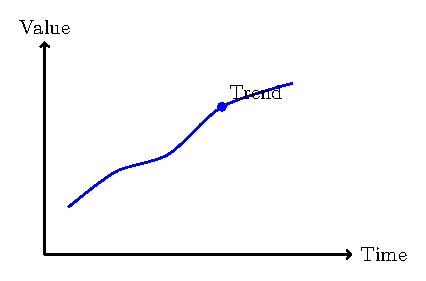
\includegraphics[width=\linewidth,height=0.48\textheight,
                         keepaspectratio]{figures/example-chart.pdf}
        \caption{面板 A：处理组}
      \end{figure}
    \column{0.48\textwidth}
      \begin{figure}
        \centering
        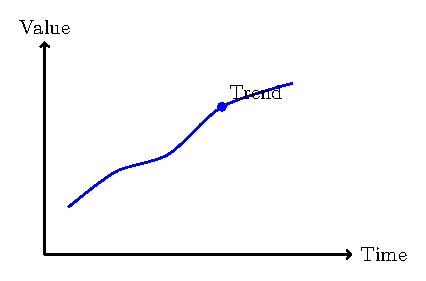
\includegraphics[width=\linewidth,height=0.48\textheight,
                         keepaspectratio]{figures/example-chart.pdf}
        \caption{面板 B：对照组}
      \end{figure}
  \end{columns}
\end{frame}

\begin{frame}{TikZ — 因果有向图 (DAG)}
  \centering
  \begin{tikzpicture}[
      node distance=1.8cm and 2.6cm,
      box/.style={draw, rounded corners=4pt,
                  minimum width=1.9cm, minimum height=0.65cm,
                  font=\small, fill=white},
      >=Stealth, thick
    ]
    \node[box] (Z) {工具变量 $Z$};
    \node[box, right=of Z] (X) {处理变量 $X$};
    \node[box, right=of X] (Y) {结果变量 $Y$};
    \node[box, dashed, above right=0.55cm and 0.9cm of X]
          (U) {不可观测 $U$};
    \draw[->] (Z) -- (X);
    \draw[->] (X) -- (Y);
    \draw[->, dashed, gray] (U) -- (X);
    \draw[->, dashed, gray] (U) -- (Y);
    \draw[->, red!70!black, bend right=18]
          node[below, font=\scriptsize, midway]{排除限制} (Z.south) to (Y.south);
    % 注：上面的 bend right 箭头演示"违反排除限制"的情形，
    %     实际使用时可删去。
  \end{tikzpicture}
  \par\smallskip
  {\footnotesize 虚线 = 不可观测路径；红色弯箭头 = 违反排除限制（示意）。}
\end{frame}

\begin{frame}{TikZ — 流程图}
  \centering
  \begin{tikzpicture}[
      node distance=0.75cm,
      box/.style={draw, rounded corners=3pt,
                  minimum width=3.4cm, minimum height=0.58cm,
                  align=center, font=\small, fill=blue!5},
      dec/.style={draw, diamond, aspect=2.6,
                  minimum width=2.8cm, font=\small, fill=orange!10},
      >=Stealth, thick
    ]
    \node[box]  (data)  {原始数据};
    \node[box, below=of data]  (clean) {清洗与预处理};
    \node[dec, below=of clean] (valid) {通过质检？};
    \node[box, below=of valid] (est)   {模型估计};
    \node[box, below=of est]   (rep)   {报告结果};

    \draw[->] (data)  -- (clean);
    \draw[->] (clean) -- (valid);
    \draw[->] (valid) -- node[right, font=\scriptsize]{是} (est);
    \draw[->] (valid.west) -- ++(-1.3,0)
              |- node[left, font=\scriptsize, pos=0.22]{否} (clean.west);
    \draw[->] (est)   -- (rep);
  \end{tikzpicture}
\end{frame}
\begin{frame}{TikZ — 水平时间轴}
  \centering
  \begin{tikzpicture}[>=Stealth, thick, font=\small]
    
    % 1. 调整背景框的深度（下移至 -0.85）
    \fill[blue!15, rounded corners=2pt] (2.2,-0.55) rectangle (6.8, 0.05);
    % 2. 将“样本期间”文字下移（Y坐标从 -0.35 改为 -0.65），避开“2008”
    \node[font=\scriptsize, text=blue!60!black] at (4.5,-0.65) {样本期间};

    % 3. 绘制主时间轴和年份刻度
    \draw[->] (-0.3,0) -- (9.2,0) node[right] {年份};
    \foreach \x/\yr in {0.5/1990, 2.5/2000, 4.5/2008, 6.5/2015, 8.5/2023}{
      \draw (\x, 0.12) -- (\x,-0.12) node[below] {\yr};
    }
    
    % 4. 事件标注（上方）
    \node[above, align=center, font=\scriptsize] at (0.5, 0.22) {改革 A};
    \node[above, align=center, font=\scriptsize] at (2.5, 0.22) {改革 B};
    \node[above, align=center, font=\scriptsize, text=red!70!black]
          at (4.5, 0.22) {金融危机};
    \node[above, align=center, font=\scriptsize] at (6.5, 0.22) {政策 C};
    \node[above, align=center, font=\scriptsize] at (8.5, 0.22) {今日};
    
    % 5. 当前位置标记
    \draw[red!70!black, thick] (8.5,0.35) -- (8.5,-0.12);
    
  \end{tikzpicture}
\end{frame}
% ------------------------------------------------------------------
\subsection{表格样例 / Tables}
% ------------------------------------------------------------------

\begin{frame}{描述性统计}
  \begin{table}
  \centering
  \caption{描述性统计（Summary Statistics）}
  {\small
  \begin{tabular}{lrrrr}
    \toprule
    变量 & 均值 & 标准差 & 最小值 & 最大值 \\
    \midrule
    人均 GDP（美元）       & 12{,}450 & 3{,}821 & 5{,}200  & 24{,}100 \\
    失业率（\%）           &     6.2  &    2.1  &     1.8  &     14.3 \\
    通货膨胀率（\%）       &     3.4  &    1.9  &  $-$0.5  &     11.2 \\
    贸易开放度             &    0.68  &   0.22  &    0.12  &      1.45 \\
    城镇化率（\%）         &    56.3  &   14.7  &    22.0  &     89.4 \\
    人力资本指数           &     2.8  &    0.6  &     1.5  &      4.1 \\
    \midrule
    样本量 $N$             & \multicolumn{4}{c}{1{,}200} \\
    \bottomrule
  \end{tabular}}
  \par\smallskip
  \raggedright
  {\footnotesize \textit{注}：年度面板数据，2000--2020 年。
  样本限于人口超过 100 万的国家。}
\end{table}

\end{frame}

\begin{frame}{多列回归比较}
  \begin{table}
  \centering
  \caption{回归结果：四种设定（Regression Results）}
  {\scriptsize
  \begin{tabular}{lcccc}
    \toprule
    & (1) OLS & (2) OLS & (3) IV & (4) IV \\
    & 基准    & +控制变量 & 基准  & +控制变量 \\
    \midrule
    处理变量          & 0.125*** & 0.098**  & 0.187*** & 0.142** \\
                      & (0.031)  & (0.040)  & (0.055)  & (0.063) \\[4pt]
    对数收入          &          & 0.234*** &          & 0.211*** \\
                      &          & (0.022)  &          & (0.025) \\[4pt]
    教育年限          &          & 0.044*   &          & 0.039*  \\
                      &          & (0.024)  &          & (0.022) \\
    \midrule
    控制变量          & 否  & 是  & 否  & 是  \\
    固定效应          & 否  & 是  & 否  & 是  \\
    $N$               & 1{,}200 & 1{,}200 & 1{,}200 & 1{,}200 \\
    $R^2$             & 0.18 & 0.34 & --- & --- \\
    F 统计（弱工具）  &      &      & 18.7 & 21.3 \\
    \bottomrule
    \multicolumn{5}{l}{%
      \scriptsize
      *** $p<0.01$，** $p<0.05$，* $p<0.1$。括号内为聚类稳健标准误。}
  \end{tabular}}
\end{table}

\end{frame}

\begin{frame}[shrink=20]{双面板（Panel A / B）异质性}
  \begin{table}
  \centering
  \caption{异质性分析：双面板（Two-Panel Heterogeneity）}
  {\footnotesize
  \begin{tabular}{lcc}
    \toprule
    & (1) 低收入组 & (2) 高收入组 \\
    \midrule
    \multicolumn{3}{l}{\textit{面板 A：城市样本}} \\
    \midrule
    处理效应   & 0.142**  & 0.098*   \\
               & (0.058)  & (0.052)  \\
    控制变量   & 是       & 是       \\
    $N$        & 600      & 600      \\
    \midrule
    \multicolumn{3}{l}{\textit{面板 B：农村样本}} \\
    \midrule
    处理效应   & 0.072    & 0.031    \\
               & (0.074)  & (0.069)  \\
    控制变量   & 是       & 是       \\
    $N$        & 400      & 400      \\
    \midrule
    \multicolumn{3}{l}{\textit{面板差异（A $-$ B）}} \\
    \midrule
    差值       & 0.070    & 0.067    \\
    $p$ 值     & 0.043    & 0.061    \\
    \bottomrule
    \multicolumn{3}{l}{%
      \footnotesize ** $p<0.05$，* $p<0.1$。括号内为聚类稳健标准误。}
  \end{tabular}}
\end{table}

\end{frame}

\begin{frame}{行高亮表格（colortbl）}
  % 需要在 main.tex 中加载 \usepackage{colortbl}
  \begin{table}
    \centering
    \caption{带高亮行的表格示例}
    \begin{tabular}{lcc}
      \toprule
      变量 & 处理组 & 对照组 \\
      \midrule
      \rowcolor{yellow!30}
      GDP 增速 (\%) & 6.8 & 3.2 \\
      失业率 (\%)   & 4.1 & 7.6 \\
      \rowcolor{yellow!30}
      通货膨胀 (\%) & 2.3 & 4.8 \\
      贸易开放度    & 0.72 & 0.51 \\
      \bottomrule
    \end{tabular}
  \end{table}
  {\footnotesize \textit{注}：黄色行为核心关注变量。}
\end{frame}

% ------------------------------------------------------------------
\subsection{代码与逐字排版 / Code \& Verbatim}
% ------------------------------------------------------------------

\begin{frame}[fragile]{Python 代码（listings）}
  % 需要在 main.tex 中加载 \usepackage{listings} 并配置 \lstset
  \begin{lstlisting}[language=Python, caption={OLS 估计量（NumPy 实现）}]
import numpy as np

def ols(X, y):
    """返回 OLS 系数向量 beta_hat."""
    return np.linalg.solve(X.T @ X, X.T @ y)

# 生成模拟数据
rng  = np.random.default_rng(42)
X    = np.column_stack([np.ones(200), rng.standard_normal((200, 2))])
beta = np.array([1.0, 2.0, -0.5])
y    = X @ beta + rng.standard_normal(200)

print(ols(X, y))   # 应接近 [1, 2, -0.5]
  \end{lstlisting}
\end{frame}

\begin{frame}[fragile]{LaTeX 代码排版（lstlisting）}
  % ⚠ Beamer 限制：[fragile] 帧的内容（含 \input 子文件）里
  %   不能出现字面的 \end{frame}，否则 Beamer 预扫描会误判帧结束。
  %   解决方法：只展示帧内部代码，外层 \begin/\end{frame} 用文字说明。
  \begin{lstlisting}[language=TeX, caption={帧内叠加动画（内部代码）}]
% 以下内容放在 frame 环境内部（外层为 \begin{frame}...\end{...} 结构）：
\begin{itemize}
  \item<1-> \alert<1>{Step 1}: 建立模型
  \item<2-> \alert<2>{Step 2}: 求解均衡
  \item<3-> \alert<3>{Step 3}: 实证检验
\end{itemize}
\setbeamercovered{transparent}  % 未到场条目置灰
  \end{lstlisting}
  {\footnotesize\textit{注}：若需在代码块中展示完整帧结构（含 \texttt{\textbackslash end\{frame\}}），
  可将代码存入独立 \texttt{.tex} 文件后用 \texttt{\textbackslash lstinputlisting} 引入。}
\end{frame}

% ------------------------------------------------------------------
\subsection{特殊幻灯片与导航 / Special Slides \& Navigation}
% ------------------------------------------------------------------

\begin{frame}{章节过渡页}
  \vspace*{\fill}
  \begin{center}
    {\Large \textbf{第~\Roman{section}~部分}}\\[0.7em]
    {\large \insertsectionhead}\\[1.2em]
    {\normalsize 一句话预告本节核心内容。}
  \end{center}
  \vspace*{\fill}
\end{frame}

\begin{frame}{进度路线图（手动高亮当前节）}
  \begin{enumerate}
    \item[\checkmark] 引言
    \item[\checkmark] 背景与文献
    \item[\textbf{3.}] \textbf{模型} \quad \textcolor{blue}{$\leftarrow$ 当前}
    \item[4.] \textcolor{gray}{实证分析}
    \item[5.] \textcolor{gray}{结论}
  \end{enumerate}
\end{frame}

\begin{frame}{两箱对比（alertblock vs exampleblock）}
  \begin{columns}[T]
    \column{0.48\textwidth}
      \begin{alertblock}{无干预（基准）}
        \begin{itemize}
          \item 产出增速：低
          \item 失业率：高
          \item 社会福利：$W_0$
        \end{itemize}
      \end{alertblock}
    \column{0.48\textwidth}
      \begin{exampleblock}{有干预（反事实）}
        \begin{itemize}
          \item 产出增速：高
          \item 失业率：低
          \item 社会福利：$W_1 > W_0$
        \end{itemize}
      \end{exampleblock}
  \end{columns}
\end{frame}

\begin{frame}{引言页 / Pull Quote}
  \vspace*{\fill}
  \begin{center}
    \Large\itshape
    ``好的模型不求包罗万象，\\
    只求能对关键机制给出清晰预测。''
    \vspace{0.9em}

    \normalsize\upshape
    --- 示例引用，\textit{来源书目}，年份
  \end{center}
  \vspace*{\fill}
\end{frame}

% 超链接导航示例
% 用法：目标帧内加 \label{frm:target}，此处用 \hyperlink{frm:target}{按钮}
\begin{frame}{附录跳转按钮}
  正文幻灯片可加入指向附录的按钮，听众提问时快速跳转：

  \medskip
  \hyperlink{frm:robustness}{\beamergotobutton{稳健性检验}}
  \hspace{1em}
  \hyperlink{frm:derivation}{\beamergotobutton{完整推导}}
  \hspace{1em}
  \hyperlink{frm:data}{\beamergotobutton{数据说明}}

  \bigskip
  附录帧返回正文：

  \medskip
  \hyperlink{frm:main-results}{\beamerreturnbutton{返回主结果}}
  \hspace{1em}
  \hyperlink{frm:empirics}{\beamerbutton{跳至实证节}}

  \bigskip
  {\footnotesize \textit{用法}：在目标帧内加
    \texttt{\textbackslash label\{frm:robustness\}} 等标签即可激活以上按钮。}
\end{frame}

%  即可将本库编译进文档。
% ============================================================

\section{Slide Gallery}

% ------------------------------------------------------------------
\subsection{文字与列表 / Text \& Lists}
% ------------------------------------------------------------------

\begin{frame}{Itemize — 三级嵌套}
  \begin{itemize}
    \item 一级条目（默认样式）
      \begin{itemize}
        \item 二级条目（缩进更深）
          \begin{itemize}
            \item 三级条目（通常避免超过三级）
          \end{itemize}
      \end{itemize}
    \item 另一条一级条目
    \item 再一条一级条目
  \end{itemize}
\end{frame}

\begin{frame}{Enumerate — 有序列表}
  \begin{enumerate}
    \item 第一步：提出问题
    \item 第二步：建立模型
      \begin{enumerate}
        \item 子步骤 A
        \item 子步骤 B
      \end{enumerate}
    \item 第三步：实证检验
    \item 第四步：政策含义
  \end{enumerate}
\end{frame}

\begin{frame}{Description — 术语表}
  \begin{description}
    \item[识别 (Identification)] 将因果效应与相关性分离的策略。
    \item[工具变量 (IV)] 影响处理变量但不直接影响结果的变量。
    \item[排除限制 (Exclusion)] 工具变量仅通过处理变量影响结果。
    \item[外生性 (Exogeneity)] 工具变量与误差项不相关的假设。
  \end{description}
\end{frame}

\begin{frame}{强调与颜色}
  \begin{itemize}
    \item 使用 \alert{alert} 将关键词标红（beamer 默认强调色）。
    \item 使用 \textbf{粗体}表示重要概念。
    \item 使用 \textit{斜体}表示书名、外文词汇。
    \item 使用 \textcolor{blue}{自定义颜色}：\texttt{\textbackslash textcolor\{blue\}\{...\}}。
    \item 使用 \colorbox{yellow!40}{背景高亮}：\texttt{\textbackslash colorbox\{yellow!40\}\{...\}}。
    \item \structure{结构色}（beamer \texttt{\textbackslash structure}）跟随主题变化。
  \end{itemize}
\end{frame}

% ------------------------------------------------------------------
\subsection{分栏布局 / Column Layouts}
% ------------------------------------------------------------------

\begin{frame}{两栏均等 50/50}
  \begin{columns}[T]
    \column{0.5\textwidth}
      \textbf{左栏}
      \begin{itemize}
        \item 论点一
        \item 论点二
        \item 论点三
      \end{itemize}
    \column{0.5\textwidth}
      \textbf{右栏}
      \begin{itemize}
        \item 反驳一
        \item 反驳二
        \item 反驳三
      \end{itemize}
  \end{columns}
\end{frame}

\begin{frame}{两栏不等 60/40（文字 + 图）}
  \begin{columns}[T]
    \column{0.60\textwidth}
      \begin{itemize}
        \item 宽栏放主要论述，窄栏放配图或摘要。
        \item 保持每条 bullet 简短，避免折行过多。
        \item 此布局适合"文字驱动"幻灯片。
      \end{itemize}
    \column{0.40\textwidth}
      \centering
      
\includegraphics[width=\linewidth]{figures/example-diagram.pdf}
      \par\smallskip
      {\tiny 图注：替换为实际图形。}
  \end{columns}
\end{frame}

\begin{frame}{三栏等宽}
  \begin{columns}[T]
    \column{0.33\textwidth}
      \centering
      \textbf{阶段一}\\[6pt]
      描述第一阶段的核心特征或数据。
    \column{0.33\textwidth}
      \centering
      \textbf{阶段二}\\[6pt]
      描述第二阶段的核心特征或数据。
    \column{0.34\textwidth}
      \centering
      \textbf{阶段三}\\[6pt]
      描述第三阶段的核心特征或数据。
  \end{columns}
\end{frame}

% ------------------------------------------------------------------
\subsection{块与定理 / Blocks \& Theorems}
% ------------------------------------------------------------------

\begin{frame}{三种标准块}
  \begin{block}{标准块 (block)}
    用于关键事实、定义、或中性信息。
  \end{block}
  \begin{alertblock}{警示块 (alertblock)}
    用于警告、重要假设、或关键局限性。
  \end{alertblock}
  \begin{exampleblock}{示例块 (exampleblock)}
    用于数值例子、实证事实、或直觉说明。
  \end{exampleblock}
\end{frame}

\begin{frame}{定理与推论}
  \begin{theorem}[包络定理]
    设 $V(\theta) = \max_x f(x, \theta)$，则
    $\dfrac{dV}{d\theta} = \dfrac{\partial f}{\partial \theta}\big|_{x=x^*(\theta)}$。
  \end{theorem}
  \begin{corollary}
    在可微条件下，值函数关于参数的单调性由 $\partial f/\partial\theta$ 的符号决定。
  \end{corollary}
\end{frame}

\begin{frame}{定义与引理}
  \begin{definition}[纳什均衡]
    策略组合 $\sigma^*$ 是纳什均衡，当且仅当对任意参与人 $i$，
    在其他人策略不变的情况下，$i$ 无法通过单边偏离获益。
  \end{definition}
  \begin{lemma}
    任何有限博弈在混合策略意义下至少存在一个纳什均衡。
  \end{lemma}
\end{frame}

\begin{frame}{证明框架}
  \begin{proof}
    设 $x^* \notin \arg\max f(x)$，则存在 $x'$ 使得 $f(x') > f(x^*)$，
    与 $x^*$ 的最优性矛盾。故 $x^*$ 确为最大值点。
  \end{proof}
  \medskip
  \begin{exampleblock}{规范说明}
    Beamer 自动在 proof 结尾添加 $\square$，无需手动输入。
  \end{exampleblock}
\end{frame}

% ------------------------------------------------------------------
\subsection{数学公式 / Math}
% ------------------------------------------------------------------

\begin{frame}{行内与独行公式}
  行内公式：$\hat{\beta} = (X^\top X)^{-1} X^\top y$，
  或 $\text{plim}\,\hat{\beta} = \beta + (X^\top X/n)^{-1}(X^\top \varepsilon/n)$。

  \[
    \sigma^2 = \frac{1}{n}\sum_{i=1}^{n}(x_i - \bar{x})^2, \qquad
    \bar{x} = \frac{1}{n}\sum_{i=1}^{n} x_i.
  \]
\end{frame}

\begin{frame}{Align 带编号}
  \begin{align}
    \ell(\beta) &= \sum_{i=1}^{n}
      \bigl[y_i \log p_i + (1-y_i)\log(1-p_i)\bigr], \label{eq:loglik} \\
    \frac{\partial \ell}{\partial \beta} &= X^\top(y - p) = 0. \label{eq:foc}
  \end{align}
  式 \eqref{eq:loglik} 为对数似然；式 \eqref{eq:foc} 为一阶条件。
\end{frame}

\begin{frame}{矩阵}
  \[
    A = \begin{pmatrix} a_{11} & a_{12} \\ a_{21} & a_{22} \end{pmatrix}, \qquad
    B = \begin{bmatrix} 1 & 0 & 0 \\ 0 & 1 & 0 \\ 0 & 0 & 1 \end{bmatrix}, \qquad
    \det(A) = a_{11}a_{22} - a_{12}a_{21}.
  \]
\end{frame}

\begin{frame}{分段函数与 Cases}
  \[
    f(x) = \begin{cases}
      \alpha + \beta x   & \text{若 } x \geq \bar{x}, \\[4pt]
      \gamma + \delta x  & \text{若 } x < \bar{x}.
    \end{cases}
  \]
  \medskip
  注：用 \texttt{\\[4pt]} 在 cases 各行之间增加垂直间距。
\end{frame}

\begin{frame}{优化问题}
  \[
    \max_{\{c_t,\,k_{t+1}\}_{t=0}^{\infty}}
    \sum_{t=0}^{\infty} \beta^t u(c_t)
  \]
  \[
    \text{s.t.} \quad c_t + k_{t+1} = A k_t^\alpha, \quad
    c_t \geq 0, \quad k_0 \text{ 给定}.
  \]
  \begin{itemize}
    \item $\beta \in (0,1)$：折现因子；\quad $\alpha \in (0,1)$：资本份额。
    \item 贝尔曼方程：$V(k) = \max_{k'} \bigl\{u(Ak^\alpha - k') + \beta V(k')\bigr\}$。
  \end{itemize}
\end{frame}

% ------------------------------------------------------------------
\subsection{叠加动画 / Overlays \& Animations}
% ------------------------------------------------------------------

\begin{frame}{逐步显示：\texttt{\textbackslash pause}}
  \begin{itemize}
    \item 第一条：出现在第 1 页。
    \pause
    \item 第二条：出现在第 2 页。
    \pause
    \item 第三条：出现在第 3 页。
  \end{itemize}
  \pause
  \begin{exampleblock}{小结（第 4 页）}
    结合具体内容决定在何处插入 \texttt{\textbackslash pause}。
  \end{exampleblock}
\end{frame}

\begin{frame}{条件替换：\texttt{\textbackslash only}}
  \only<1>{
    \begin{block}{步骤 1 — 建模}
      定义参与人、策略空间和支付函数。
    \end{block}
  }
  \only<2>{
    \begin{block}{步骤 2 — 求解}
      对每位参与人求最优反应函数，联立求解。
    \end{block}
  }
  \only<3>{
    \begin{block}{步骤 3 — 解读}
      分析均衡的经济含义与福利性质。
    \end{block}
  }
  \vspace{0.5cm}
  \centering\footnotesize
  [\only<1>{第 1/3 页}\only<2>{第 2/3 页}\only<3>{第 3/3 页}]
\end{frame}

\begin{frame}{关键词逐步高亮：\texttt{\textbackslash alert<>}}
  估计策略分三步：
  \begin{itemize}
    \item<1-> \alert<1>{识别}：利用准随机变异剥离内生性。
    \item<2-> \alert<2>{估计}：对简约式做 OLS，获得降维方程。
    \item<3-> \alert<3>{推断}：使用聚类稳健标准误进行显著性检验。
  \end{itemize}
\end{frame}

\begin{frame}{未来条目置灰：\texttt{transparent}}
  {%  使用大括号将效果限制在本帧
    \setbeamercovered{transparent}
    \begin{itemize}
      \item<1-> 条目一（第 1 页完全可见，后续置灰）
      \item<2-> 条目二（第 2 页完全可见）
      \item<3-> 条目三（第 3 页完全可见）
    \end{itemize}
  }
\end{frame}

% ------------------------------------------------------------------
\subsection{图形与 TikZ / Figures \& TikZ}
% ------------------------------------------------------------------

\begin{frame}{并排双图（minipage）}
  \begin{columns}[c]
    \column{0.48\textwidth}
      \begin{figure}
        \centering
        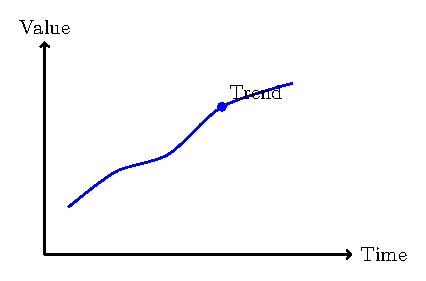
\includegraphics[width=\linewidth,height=0.48\textheight,
                         keepaspectratio]{figures/example-chart.pdf}
        \caption{面板 A：处理组}
      \end{figure}
    \column{0.48\textwidth}
      \begin{figure}
        \centering
        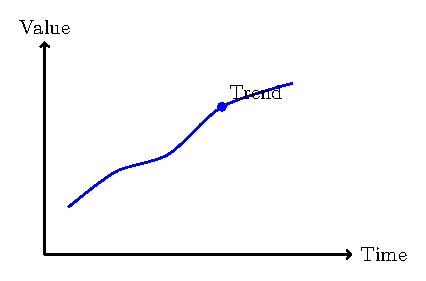
\includegraphics[width=\linewidth,height=0.48\textheight,
                         keepaspectratio]{figures/example-chart.pdf}
        \caption{面板 B：对照组}
      \end{figure}
  \end{columns}
\end{frame}

\begin{frame}{TikZ — 因果有向图 (DAG)}
  \centering
  \begin{tikzpicture}[
      node distance=1.8cm and 2.6cm,
      box/.style={draw, rounded corners=4pt,
                  minimum width=1.9cm, minimum height=0.65cm,
                  font=\small, fill=white},
      >=Stealth, thick
    ]
    \node[box] (Z) {工具变量 $Z$};
    \node[box, right=of Z] (X) {处理变量 $X$};
    \node[box, right=of X] (Y) {结果变量 $Y$};
    \node[box, dashed, above right=0.55cm and 0.9cm of X]
          (U) {不可观测 $U$};
    \draw[->] (Z) -- (X);
    \draw[->] (X) -- (Y);
    \draw[->, dashed, gray] (U) -- (X);
    \draw[->, dashed, gray] (U) -- (Y);
    \draw[->, red!70!black, bend right=18]
          node[below, font=\scriptsize, midway]{排除限制} (Z.south) to (Y.south);
    % 注：上面的 bend right 箭头演示"违反排除限制"的情形，
    %     实际使用时可删去。
  \end{tikzpicture}
  \par\smallskip
  {\footnotesize 虚线 = 不可观测路径；红色弯箭头 = 违反排除限制（示意）。}
\end{frame}

\begin{frame}{TikZ — 流程图}
  \centering
  \begin{tikzpicture}[
      node distance=0.75cm,
      box/.style={draw, rounded corners=3pt,
                  minimum width=3.4cm, minimum height=0.58cm,
                  align=center, font=\small, fill=blue!5},
      dec/.style={draw, diamond, aspect=2.6,
                  minimum width=2.8cm, font=\small, fill=orange!10},
      >=Stealth, thick
    ]
    \node[box]  (data)  {原始数据};
    \node[box, below=of data]  (clean) {清洗与预处理};
    \node[dec, below=of clean] (valid) {通过质检？};
    \node[box, below=of valid] (est)   {模型估计};
    \node[box, below=of est]   (rep)   {报告结果};

    \draw[->] (data)  -- (clean);
    \draw[->] (clean) -- (valid);
    \draw[->] (valid) -- node[right, font=\scriptsize]{是} (est);
    \draw[->] (valid.west) -- ++(-1.3,0)
              |- node[left, font=\scriptsize, pos=0.22]{否} (clean.west);
    \draw[->] (est)   -- (rep);
  \end{tikzpicture}
\end{frame}
\begin{frame}{TikZ — 水平时间轴}
  \centering
  \begin{tikzpicture}[>=Stealth, thick, font=\small]
    
    % 1. 调整背景框的深度（下移至 -0.85）
    \fill[blue!15, rounded corners=2pt] (2.2,-0.55) rectangle (6.8, 0.05);
    % 2. 将“样本期间”文字下移（Y坐标从 -0.35 改为 -0.65），避开“2008”
    \node[font=\scriptsize, text=blue!60!black] at (4.5,-0.65) {样本期间};

    % 3. 绘制主时间轴和年份刻度
    \draw[->] (-0.3,0) -- (9.2,0) node[right] {年份};
    \foreach \x/\yr in {0.5/1990, 2.5/2000, 4.5/2008, 6.5/2015, 8.5/2023}{
      \draw (\x, 0.12) -- (\x,-0.12) node[below] {\yr};
    }
    
    % 4. 事件标注（上方）
    \node[above, align=center, font=\scriptsize] at (0.5, 0.22) {改革 A};
    \node[above, align=center, font=\scriptsize] at (2.5, 0.22) {改革 B};
    \node[above, align=center, font=\scriptsize, text=red!70!black]
          at (4.5, 0.22) {金融危机};
    \node[above, align=center, font=\scriptsize] at (6.5, 0.22) {政策 C};
    \node[above, align=center, font=\scriptsize] at (8.5, 0.22) {今日};
    
    % 5. 当前位置标记
    \draw[red!70!black, thick] (8.5,0.35) -- (8.5,-0.12);
    
  \end{tikzpicture}
\end{frame}
% ------------------------------------------------------------------
\subsection{表格样例 / Tables}
% ------------------------------------------------------------------

\begin{frame}{描述性统计}
  \begin{table}
  \centering
  \caption{描述性统计（Summary Statistics）}
  {\small
  \begin{tabular}{lrrrr}
    \toprule
    变量 & 均值 & 标准差 & 最小值 & 最大值 \\
    \midrule
    人均 GDP（美元）       & 12{,}450 & 3{,}821 & 5{,}200  & 24{,}100 \\
    失业率（\%）           &     6.2  &    2.1  &     1.8  &     14.3 \\
    通货膨胀率（\%）       &     3.4  &    1.9  &  $-$0.5  &     11.2 \\
    贸易开放度             &    0.68  &   0.22  &    0.12  &      1.45 \\
    城镇化率（\%）         &    56.3  &   14.7  &    22.0  &     89.4 \\
    人力资本指数           &     2.8  &    0.6  &     1.5  &      4.1 \\
    \midrule
    样本量 $N$             & \multicolumn{4}{c}{1{,}200} \\
    \bottomrule
  \end{tabular}}
  \par\smallskip
  \raggedright
  {\footnotesize \textit{注}：年度面板数据，2000--2020 年。
  样本限于人口超过 100 万的国家。}
\end{table}

\end{frame}

\begin{frame}{多列回归比较}
  \begin{table}
  \centering
  \caption{回归结果：四种设定（Regression Results）}
  {\scriptsize
  \begin{tabular}{lcccc}
    \toprule
    & (1) OLS & (2) OLS & (3) IV & (4) IV \\
    & 基准    & +控制变量 & 基准  & +控制变量 \\
    \midrule
    处理变量          & 0.125*** & 0.098**  & 0.187*** & 0.142** \\
                      & (0.031)  & (0.040)  & (0.055)  & (0.063) \\[4pt]
    对数收入          &          & 0.234*** &          & 0.211*** \\
                      &          & (0.022)  &          & (0.025) \\[4pt]
    教育年限          &          & 0.044*   &          & 0.039*  \\
                      &          & (0.024)  &          & (0.022) \\
    \midrule
    控制变量          & 否  & 是  & 否  & 是  \\
    固定效应          & 否  & 是  & 否  & 是  \\
    $N$               & 1{,}200 & 1{,}200 & 1{,}200 & 1{,}200 \\
    $R^2$             & 0.18 & 0.34 & --- & --- \\
    F 统计（弱工具）  &      &      & 18.7 & 21.3 \\
    \bottomrule
    \multicolumn{5}{l}{%
      \scriptsize
      *** $p<0.01$，** $p<0.05$，* $p<0.1$。括号内为聚类稳健标准误。}
  \end{tabular}}
\end{table}

\end{frame}

\begin{frame}[shrink=20]{双面板（Panel A / B）异质性}
  \begin{table}
  \centering
  \caption{异质性分析：双面板（Two-Panel Heterogeneity）}
  {\footnotesize
  \begin{tabular}{lcc}
    \toprule
    & (1) 低收入组 & (2) 高收入组 \\
    \midrule
    \multicolumn{3}{l}{\textit{面板 A：城市样本}} \\
    \midrule
    处理效应   & 0.142**  & 0.098*   \\
               & (0.058)  & (0.052)  \\
    控制变量   & 是       & 是       \\
    $N$        & 600      & 600      \\
    \midrule
    \multicolumn{3}{l}{\textit{面板 B：农村样本}} \\
    \midrule
    处理效应   & 0.072    & 0.031    \\
               & (0.074)  & (0.069)  \\
    控制变量   & 是       & 是       \\
    $N$        & 400      & 400      \\
    \midrule
    \multicolumn{3}{l}{\textit{面板差异（A $-$ B）}} \\
    \midrule
    差值       & 0.070    & 0.067    \\
    $p$ 值     & 0.043    & 0.061    \\
    \bottomrule
    \multicolumn{3}{l}{%
      \footnotesize ** $p<0.05$，* $p<0.1$。括号内为聚类稳健标准误。}
  \end{tabular}}
\end{table}

\end{frame}

\begin{frame}{行高亮表格（colortbl）}
  % 需要在 main.tex 中加载 \usepackage{colortbl}
  \begin{table}
    \centering
    \caption{带高亮行的表格示例}
    \begin{tabular}{lcc}
      \toprule
      变量 & 处理组 & 对照组 \\
      \midrule
      \rowcolor{yellow!30}
      GDP 增速 (\%) & 6.8 & 3.2 \\
      失业率 (\%)   & 4.1 & 7.6 \\
      \rowcolor{yellow!30}
      通货膨胀 (\%) & 2.3 & 4.8 \\
      贸易开放度    & 0.72 & 0.51 \\
      \bottomrule
    \end{tabular}
  \end{table}
  {\footnotesize \textit{注}：黄色行为核心关注变量。}
\end{frame}

% ------------------------------------------------------------------
\subsection{代码与逐字排版 / Code \& Verbatim}
% ------------------------------------------------------------------

\begin{frame}[fragile]{Python 代码（listings）}
  % 需要在 main.tex 中加载 \usepackage{listings} 并配置 \lstset
  \begin{lstlisting}[language=Python, caption={OLS 估计量（NumPy 实现）}]
import numpy as np

def ols(X, y):
    """返回 OLS 系数向量 beta_hat."""
    return np.linalg.solve(X.T @ X, X.T @ y)

# 生成模拟数据
rng  = np.random.default_rng(42)
X    = np.column_stack([np.ones(200), rng.standard_normal((200, 2))])
beta = np.array([1.0, 2.0, -0.5])
y    = X @ beta + rng.standard_normal(200)

print(ols(X, y))   # 应接近 [1, 2, -0.5]
  \end{lstlisting}
\end{frame}

\begin{frame}[fragile]{LaTeX 代码排版（lstlisting）}
  % ⚠ Beamer 限制：[fragile] 帧的内容（含 \input 子文件）里
  %   不能出现字面的 \end{frame}，否则 Beamer 预扫描会误判帧结束。
  %   解决方法：只展示帧内部代码，外层 \begin/\end{frame} 用文字说明。
  \begin{lstlisting}[language=TeX, caption={帧内叠加动画（内部代码）}]
% 以下内容放在 frame 环境内部（外层为 \begin{frame}...\end{...} 结构）：
\begin{itemize}
  \item<1-> \alert<1>{Step 1}: 建立模型
  \item<2-> \alert<2>{Step 2}: 求解均衡
  \item<3-> \alert<3>{Step 3}: 实证检验
\end{itemize}
\setbeamercovered{transparent}  % 未到场条目置灰
  \end{lstlisting}
  {\footnotesize\textit{注}：若需在代码块中展示完整帧结构（含 \texttt{\textbackslash end\{frame\}}），
  可将代码存入独立 \texttt{.tex} 文件后用 \texttt{\textbackslash lstinputlisting} 引入。}
\end{frame}

% ------------------------------------------------------------------
\subsection{特殊幻灯片与导航 / Special Slides \& Navigation}
% ------------------------------------------------------------------

\begin{frame}{章节过渡页}
  \vspace*{\fill}
  \begin{center}
    {\Large \textbf{第~\Roman{section}~部分}}\\[0.7em]
    {\large \insertsectionhead}\\[1.2em]
    {\normalsize 一句话预告本节核心内容。}
  \end{center}
  \vspace*{\fill}
\end{frame}

\begin{frame}{进度路线图（手动高亮当前节）}
  \begin{enumerate}
    \item[\checkmark] 引言
    \item[\checkmark] 背景与文献
    \item[\textbf{3.}] \textbf{模型} \quad \textcolor{blue}{$\leftarrow$ 当前}
    \item[4.] \textcolor{gray}{实证分析}
    \item[5.] \textcolor{gray}{结论}
  \end{enumerate}
\end{frame}

\begin{frame}{两箱对比（alertblock vs exampleblock）}
  \begin{columns}[T]
    \column{0.48\textwidth}
      \begin{alertblock}{无干预（基准）}
        \begin{itemize}
          \item 产出增速：低
          \item 失业率：高
          \item 社会福利：$W_0$
        \end{itemize}
      \end{alertblock}
    \column{0.48\textwidth}
      \begin{exampleblock}{有干预（反事实）}
        \begin{itemize}
          \item 产出增速：高
          \item 失业率：低
          \item 社会福利：$W_1 > W_0$
        \end{itemize}
      \end{exampleblock}
  \end{columns}
\end{frame}

\begin{frame}{引言页 / Pull Quote}
  \vspace*{\fill}
  \begin{center}
    \Large\itshape
    ``好的模型不求包罗万象，\\
    只求能对关键机制给出清晰预测。''
    \vspace{0.9em}

    \normalsize\upshape
    --- 示例引用，\textit{来源书目}，年份
  \end{center}
  \vspace*{\fill}
\end{frame}

% 超链接导航示例
% 用法：目标帧内加 \label{frm:target}，此处用 \hyperlink{frm:target}{按钮}
\begin{frame}{附录跳转按钮}
  正文幻灯片可加入指向附录的按钮，听众提问时快速跳转：

  \medskip
  \hyperlink{frm:robustness}{\beamergotobutton{稳健性检验}}
  \hspace{1em}
  \hyperlink{frm:derivation}{\beamergotobutton{完整推导}}
  \hspace{1em}
  \hyperlink{frm:data}{\beamergotobutton{数据说明}}

  \bigskip
  附录帧返回正文：

  \medskip
  \hyperlink{frm:main-results}{\beamerreturnbutton{返回主结果}}
  \hspace{1em}
  \hyperlink{frm:empirics}{\beamerbutton{跳至实证节}}

  \bigskip
  {\footnotesize \textit{用法}：在目标帧内加
    \texttt{\textbackslash label\{frm:robustness\}} 等标签即可激活以上按钮。}
\end{frame}

%  即可将本库编译进文档。
% ============================================================

\section{Slide Gallery}

% ------------------------------------------------------------------
\subsection{文字与列表 / Text \& Lists}
% ------------------------------------------------------------------

\begin{frame}{Itemize — 三级嵌套}
  \begin{itemize}
    \item 一级条目（默认样式）
      \begin{itemize}
        \item 二级条目（缩进更深）
          \begin{itemize}
            \item 三级条目（通常避免超过三级）
          \end{itemize}
      \end{itemize}
    \item 另一条一级条目
    \item 再一条一级条目
  \end{itemize}
\end{frame}

\begin{frame}{Enumerate — 有序列表}
  \begin{enumerate}
    \item 第一步：提出问题
    \item 第二步：建立模型
      \begin{enumerate}
        \item 子步骤 A
        \item 子步骤 B
      \end{enumerate}
    \item 第三步：实证检验
    \item 第四步：政策含义
  \end{enumerate}
\end{frame}

\begin{frame}{Description — 术语表}
  \begin{description}
    \item[识别 (Identification)] 将因果效应与相关性分离的策略。
    \item[工具变量 (IV)] 影响处理变量但不直接影响结果的变量。
    \item[排除限制 (Exclusion)] 工具变量仅通过处理变量影响结果。
    \item[外生性 (Exogeneity)] 工具变量与误差项不相关的假设。
  \end{description}
\end{frame}

\begin{frame}{强调与颜色}
  \begin{itemize}
    \item 使用 \alert{alert} 将关键词标红（beamer 默认强调色）。
    \item 使用 \textbf{粗体}表示重要概念。
    \item 使用 \textit{斜体}表示书名、外文词汇。
    \item 使用 \textcolor{blue}{自定义颜色}：\texttt{\textbackslash textcolor\{blue\}\{...\}}。
    \item 使用 \colorbox{yellow!40}{背景高亮}：\texttt{\textbackslash colorbox\{yellow!40\}\{...\}}。
    \item \structure{结构色}（beamer \texttt{\textbackslash structure}）跟随主题变化。
  \end{itemize}
\end{frame}

% ------------------------------------------------------------------
\subsection{分栏布局 / Column Layouts}
% ------------------------------------------------------------------

\begin{frame}{两栏均等 50/50}
  \begin{columns}[T]
    \column{0.5\textwidth}
      \textbf{左栏}
      \begin{itemize}
        \item 论点一
        \item 论点二
        \item 论点三
      \end{itemize}
    \column{0.5\textwidth}
      \textbf{右栏}
      \begin{itemize}
        \item 反驳一
        \item 反驳二
        \item 反驳三
      \end{itemize}
  \end{columns}
\end{frame}

\begin{frame}{两栏不等 60/40（文字 + 图）}
  \begin{columns}[T]
    \column{0.60\textwidth}
      \begin{itemize}
        \item 宽栏放主要论述，窄栏放配图或摘要。
        \item 保持每条 bullet 简短，避免折行过多。
        \item 此布局适合"文字驱动"幻灯片。
      \end{itemize}
    \column{0.40\textwidth}
      \centering
      
\includegraphics[width=\linewidth]{figures/example-diagram.pdf}
      \par\smallskip
      {\tiny 图注：替换为实际图形。}
  \end{columns}
\end{frame}

\begin{frame}{三栏等宽}
  \begin{columns}[T]
    \column{0.33\textwidth}
      \centering
      \textbf{阶段一}\\[6pt]
      描述第一阶段的核心特征或数据。
    \column{0.33\textwidth}
      \centering
      \textbf{阶段二}\\[6pt]
      描述第二阶段的核心特征或数据。
    \column{0.34\textwidth}
      \centering
      \textbf{阶段三}\\[6pt]
      描述第三阶段的核心特征或数据。
  \end{columns}
\end{frame}

% ------------------------------------------------------------------
\subsection{块与定理 / Blocks \& Theorems}
% ------------------------------------------------------------------

\begin{frame}{三种标准块}
  \begin{block}{标准块 (block)}
    用于关键事实、定义、或中性信息。
  \end{block}
  \begin{alertblock}{警示块 (alertblock)}
    用于警告、重要假设、或关键局限性。
  \end{alertblock}
  \begin{exampleblock}{示例块 (exampleblock)}
    用于数值例子、实证事实、或直觉说明。
  \end{exampleblock}
\end{frame}

\begin{frame}{定理与推论}
  \begin{theorem}[包络定理]
    设 $V(\theta) = \max_x f(x, \theta)$，则
    $\dfrac{dV}{d\theta} = \dfrac{\partial f}{\partial \theta}\big|_{x=x^*(\theta)}$。
  \end{theorem}
  \begin{corollary}
    在可微条件下，值函数关于参数的单调性由 $\partial f/\partial\theta$ 的符号决定。
  \end{corollary}
\end{frame}

\begin{frame}{定义与引理}
  \begin{definition}[纳什均衡]
    策略组合 $\sigma^*$ 是纳什均衡，当且仅当对任意参与人 $i$，
    在其他人策略不变的情况下，$i$ 无法通过单边偏离获益。
  \end{definition}
  \begin{lemma}
    任何有限博弈在混合策略意义下至少存在一个纳什均衡。
  \end{lemma}
\end{frame}

\begin{frame}{证明框架}
  \begin{proof}
    设 $x^* \notin \arg\max f(x)$，则存在 $x'$ 使得 $f(x') > f(x^*)$，
    与 $x^*$ 的最优性矛盾。故 $x^*$ 确为最大值点。
  \end{proof}
  \medskip
  \begin{exampleblock}{规范说明}
    Beamer 自动在 proof 结尾添加 $\square$，无需手动输入。
  \end{exampleblock}
\end{frame}

% ------------------------------------------------------------------
\subsection{数学公式 / Math}
% ------------------------------------------------------------------

\begin{frame}{行内与独行公式}
  行内公式：$\hat{\beta} = (X^\top X)^{-1} X^\top y$，
  或 $\text{plim}\,\hat{\beta} = \beta + (X^\top X/n)^{-1}(X^\top \varepsilon/n)$。

  \[
    \sigma^2 = \frac{1}{n}\sum_{i=1}^{n}(x_i - \bar{x})^2, \qquad
    \bar{x} = \frac{1}{n}\sum_{i=1}^{n} x_i.
  \]
\end{frame}

\begin{frame}{Align 带编号}
  \begin{align}
    \ell(\beta) &= \sum_{i=1}^{n}
      \bigl[y_i \log p_i + (1-y_i)\log(1-p_i)\bigr], \label{eq:loglik} \\
    \frac{\partial \ell}{\partial \beta} &= X^\top(y - p) = 0. \label{eq:foc}
  \end{align}
  式 \eqref{eq:loglik} 为对数似然；式 \eqref{eq:foc} 为一阶条件。
\end{frame}

\begin{frame}{矩阵}
  \[
    A = \begin{pmatrix} a_{11} & a_{12} \\ a_{21} & a_{22} \end{pmatrix}, \qquad
    B = \begin{bmatrix} 1 & 0 & 0 \\ 0 & 1 & 0 \\ 0 & 0 & 1 \end{bmatrix}, \qquad
    \det(A) = a_{11}a_{22} - a_{12}a_{21}.
  \]
\end{frame}

\begin{frame}{分段函数与 Cases}
  \[
    f(x) = \begin{cases}
      \alpha + \beta x   & \text{若 } x \geq \bar{x}, \\[4pt]
      \gamma + \delta x  & \text{若 } x < \bar{x}.
    \end{cases}
  \]
  \medskip
  注：用 \texttt{\\[4pt]} 在 cases 各行之间增加垂直间距。
\end{frame}

\begin{frame}{优化问题}
  \[
    \max_{\{c_t,\,k_{t+1}\}_{t=0}^{\infty}}
    \sum_{t=0}^{\infty} \beta^t u(c_t)
  \]
  \[
    \text{s.t.} \quad c_t + k_{t+1} = A k_t^\alpha, \quad
    c_t \geq 0, \quad k_0 \text{ 给定}.
  \]
  \begin{itemize}
    \item $\beta \in (0,1)$：折现因子；\quad $\alpha \in (0,1)$：资本份额。
    \item 贝尔曼方程：$V(k) = \max_{k'} \bigl\{u(Ak^\alpha - k') + \beta V(k')\bigr\}$。
  \end{itemize}
\end{frame}

% ------------------------------------------------------------------
\subsection{叠加动画 / Overlays \& Animations}
% ------------------------------------------------------------------

\begin{frame}{逐步显示：\texttt{\textbackslash pause}}
  \begin{itemize}
    \item 第一条：出现在第 1 页。
    \pause
    \item 第二条：出现在第 2 页。
    \pause
    \item 第三条：出现在第 3 页。
  \end{itemize}
  \pause
  \begin{exampleblock}{小结（第 4 页）}
    结合具体内容决定在何处插入 \texttt{\textbackslash pause}。
  \end{exampleblock}
\end{frame}

\begin{frame}{条件替换：\texttt{\textbackslash only}}
  \only<1>{
    \begin{block}{步骤 1 — 建模}
      定义参与人、策略空间和支付函数。
    \end{block}
  }
  \only<2>{
    \begin{block}{步骤 2 — 求解}
      对每位参与人求最优反应函数，联立求解。
    \end{block}
  }
  \only<3>{
    \begin{block}{步骤 3 — 解读}
      分析均衡的经济含义与福利性质。
    \end{block}
  }
  \vspace{0.5cm}
  \centering\footnotesize
  [\only<1>{第 1/3 页}\only<2>{第 2/3 页}\only<3>{第 3/3 页}]
\end{frame}

\begin{frame}{关键词逐步高亮：\texttt{\textbackslash alert<>}}
  估计策略分三步：
  \begin{itemize}
    \item<1-> \alert<1>{识别}：利用准随机变异剥离内生性。
    \item<2-> \alert<2>{估计}：对简约式做 OLS，获得降维方程。
    \item<3-> \alert<3>{推断}：使用聚类稳健标准误进行显著性检验。
  \end{itemize}
\end{frame}

\begin{frame}{未来条目置灰：\texttt{transparent}}
  {%  使用大括号将效果限制在本帧
    \setbeamercovered{transparent}
    \begin{itemize}
      \item<1-> 条目一（第 1 页完全可见，后续置灰）
      \item<2-> 条目二（第 2 页完全可见）
      \item<3-> 条目三（第 3 页完全可见）
    \end{itemize}
  }
\end{frame}

% ------------------------------------------------------------------
\subsection{图形与 TikZ / Figures \& TikZ}
% ------------------------------------------------------------------

\begin{frame}{并排双图（minipage）}
  \begin{columns}[c]
    \column{0.48\textwidth}
      \begin{figure}
        \centering
        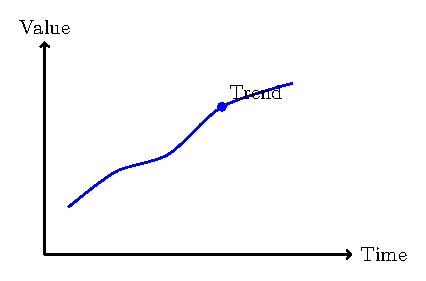
\includegraphics[width=\linewidth,height=0.48\textheight,
                         keepaspectratio]{figures/example-chart.pdf}
        \caption{面板 A：处理组}
      \end{figure}
    \column{0.48\textwidth}
      \begin{figure}
        \centering
        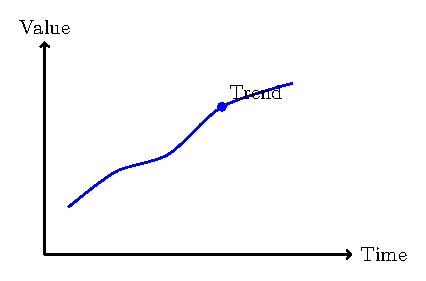
\includegraphics[width=\linewidth,height=0.48\textheight,
                         keepaspectratio]{figures/example-chart.pdf}
        \caption{面板 B：对照组}
      \end{figure}
  \end{columns}
\end{frame}

\begin{frame}{TikZ — 因果有向图 (DAG)}
  \centering
  \begin{tikzpicture}[
      node distance=1.8cm and 2.6cm,
      box/.style={draw, rounded corners=4pt,
                  minimum width=1.9cm, minimum height=0.65cm,
                  font=\small, fill=white},
      >=Stealth, thick
    ]
    \node[box] (Z) {工具变量 $Z$};
    \node[box, right=of Z] (X) {处理变量 $X$};
    \node[box, right=of X] (Y) {结果变量 $Y$};
    \node[box, dashed, above right=0.55cm and 0.9cm of X]
          (U) {不可观测 $U$};
    \draw[->] (Z) -- (X);
    \draw[->] (X) -- (Y);
    \draw[->, dashed, gray] (U) -- (X);
    \draw[->, dashed, gray] (U) -- (Y);
    \draw[->, red!70!black, bend right=18]
          node[below, font=\scriptsize, midway]{排除限制} (Z.south) to (Y.south);
    % 注：上面的 bend right 箭头演示"违反排除限制"的情形，
    %     实际使用时可删去。
  \end{tikzpicture}
  \par\smallskip
  {\footnotesize 虚线 = 不可观测路径；红色弯箭头 = 违反排除限制（示意）。}
\end{frame}

\begin{frame}{TikZ — 流程图}
  \centering
  \begin{tikzpicture}[
      node distance=0.75cm,
      box/.style={draw, rounded corners=3pt,
                  minimum width=3.4cm, minimum height=0.58cm,
                  align=center, font=\small, fill=blue!5},
      dec/.style={draw, diamond, aspect=2.6,
                  minimum width=2.8cm, font=\small, fill=orange!10},
      >=Stealth, thick
    ]
    \node[box]  (data)  {原始数据};
    \node[box, below=of data]  (clean) {清洗与预处理};
    \node[dec, below=of clean] (valid) {通过质检？};
    \node[box, below=of valid] (est)   {模型估计};
    \node[box, below=of est]   (rep)   {报告结果};

    \draw[->] (data)  -- (clean);
    \draw[->] (clean) -- (valid);
    \draw[->] (valid) -- node[right, font=\scriptsize]{是} (est);
    \draw[->] (valid.west) -- ++(-1.3,0)
              |- node[left, font=\scriptsize, pos=0.22]{否} (clean.west);
    \draw[->] (est)   -- (rep);
  \end{tikzpicture}
\end{frame}
\begin{frame}{TikZ — 水平时间轴}
  \centering
  \begin{tikzpicture}[>=Stealth, thick, font=\small]
    
    % 1. 调整背景框的深度（下移至 -0.85）
    \fill[blue!15, rounded corners=2pt] (2.2,-0.55) rectangle (6.8, 0.05);
    % 2. 将“样本期间”文字下移（Y坐标从 -0.35 改为 -0.65），避开“2008”
    \node[font=\scriptsize, text=blue!60!black] at (4.5,-0.65) {样本期间};

    % 3. 绘制主时间轴和年份刻度
    \draw[->] (-0.3,0) -- (9.2,0) node[right] {年份};
    \foreach \x/\yr in {0.5/1990, 2.5/2000, 4.5/2008, 6.5/2015, 8.5/2023}{
      \draw (\x, 0.12) -- (\x,-0.12) node[below] {\yr};
    }
    
    % 4. 事件标注（上方）
    \node[above, align=center, font=\scriptsize] at (0.5, 0.22) {改革 A};
    \node[above, align=center, font=\scriptsize] at (2.5, 0.22) {改革 B};
    \node[above, align=center, font=\scriptsize, text=red!70!black]
          at (4.5, 0.22) {金融危机};
    \node[above, align=center, font=\scriptsize] at (6.5, 0.22) {政策 C};
    \node[above, align=center, font=\scriptsize] at (8.5, 0.22) {今日};
    
    % 5. 当前位置标记
    \draw[red!70!black, thick] (8.5,0.35) -- (8.5,-0.12);
    
  \end{tikzpicture}
\end{frame}
% ------------------------------------------------------------------
\subsection{表格样例 / Tables}
% ------------------------------------------------------------------

\begin{frame}{描述性统计}
  \begin{table}
  \centering
  \caption{描述性统计（Summary Statistics）}
  {\small
  \begin{tabular}{lrrrr}
    \toprule
    变量 & 均值 & 标准差 & 最小值 & 最大值 \\
    \midrule
    人均 GDP（美元）       & 12{,}450 & 3{,}821 & 5{,}200  & 24{,}100 \\
    失业率（\%）           &     6.2  &    2.1  &     1.8  &     14.3 \\
    通货膨胀率（\%）       &     3.4  &    1.9  &  $-$0.5  &     11.2 \\
    贸易开放度             &    0.68  &   0.22  &    0.12  &      1.45 \\
    城镇化率（\%）         &    56.3  &   14.7  &    22.0  &     89.4 \\
    人力资本指数           &     2.8  &    0.6  &     1.5  &      4.1 \\
    \midrule
    样本量 $N$             & \multicolumn{4}{c}{1{,}200} \\
    \bottomrule
  \end{tabular}}
  \par\smallskip
  \raggedright
  {\footnotesize \textit{注}：年度面板数据，2000--2020 年。
  样本限于人口超过 100 万的国家。}
\end{table}

\end{frame}

\begin{frame}{多列回归比较}
  \begin{table}
  \centering
  \caption{回归结果：四种设定（Regression Results）}
  {\scriptsize
  \begin{tabular}{lcccc}
    \toprule
    & (1) OLS & (2) OLS & (3) IV & (4) IV \\
    & 基准    & +控制变量 & 基准  & +控制变量 \\
    \midrule
    处理变量          & 0.125*** & 0.098**  & 0.187*** & 0.142** \\
                      & (0.031)  & (0.040)  & (0.055)  & (0.063) \\[4pt]
    对数收入          &          & 0.234*** &          & 0.211*** \\
                      &          & (0.022)  &          & (0.025) \\[4pt]
    教育年限          &          & 0.044*   &          & 0.039*  \\
                      &          & (0.024)  &          & (0.022) \\
    \midrule
    控制变量          & 否  & 是  & 否  & 是  \\
    固定效应          & 否  & 是  & 否  & 是  \\
    $N$               & 1{,}200 & 1{,}200 & 1{,}200 & 1{,}200 \\
    $R^2$             & 0.18 & 0.34 & --- & --- \\
    F 统计（弱工具）  &      &      & 18.7 & 21.3 \\
    \bottomrule
    \multicolumn{5}{l}{%
      \scriptsize
      *** $p<0.01$，** $p<0.05$，* $p<0.1$。括号内为聚类稳健标准误。}
  \end{tabular}}
\end{table}

\end{frame}

\begin{frame}[shrink=20]{双面板（Panel A / B）异质性}
  \begin{table}
  \centering
  \caption{异质性分析：双面板（Two-Panel Heterogeneity）}
  {\footnotesize
  \begin{tabular}{lcc}
    \toprule
    & (1) 低收入组 & (2) 高收入组 \\
    \midrule
    \multicolumn{3}{l}{\textit{面板 A：城市样本}} \\
    \midrule
    处理效应   & 0.142**  & 0.098*   \\
               & (0.058)  & (0.052)  \\
    控制变量   & 是       & 是       \\
    $N$        & 600      & 600      \\
    \midrule
    \multicolumn{3}{l}{\textit{面板 B：农村样本}} \\
    \midrule
    处理效应   & 0.072    & 0.031    \\
               & (0.074)  & (0.069)  \\
    控制变量   & 是       & 是       \\
    $N$        & 400      & 400      \\
    \midrule
    \multicolumn{3}{l}{\textit{面板差异（A $-$ B）}} \\
    \midrule
    差值       & 0.070    & 0.067    \\
    $p$ 值     & 0.043    & 0.061    \\
    \bottomrule
    \multicolumn{3}{l}{%
      \footnotesize ** $p<0.05$，* $p<0.1$。括号内为聚类稳健标准误。}
  \end{tabular}}
\end{table}

\end{frame}

\begin{frame}{行高亮表格（colortbl）}
  % 需要在 main.tex 中加载 \usepackage{colortbl}
  \begin{table}
    \centering
    \caption{带高亮行的表格示例}
    \begin{tabular}{lcc}
      \toprule
      变量 & 处理组 & 对照组 \\
      \midrule
      \rowcolor{yellow!30}
      GDP 增速 (\%) & 6.8 & 3.2 \\
      失业率 (\%)   & 4.1 & 7.6 \\
      \rowcolor{yellow!30}
      通货膨胀 (\%) & 2.3 & 4.8 \\
      贸易开放度    & 0.72 & 0.51 \\
      \bottomrule
    \end{tabular}
  \end{table}
  {\footnotesize \textit{注}：黄色行为核心关注变量。}
\end{frame}

% ------------------------------------------------------------------
\subsection{代码与逐字排版 / Code \& Verbatim}
% ------------------------------------------------------------------

\begin{frame}[fragile]{Python 代码（listings）}
  % 需要在 main.tex 中加载 \usepackage{listings} 并配置 \lstset
  \begin{lstlisting}[language=Python, caption={OLS 估计量（NumPy 实现）}]
import numpy as np

def ols(X, y):
    """返回 OLS 系数向量 beta_hat."""
    return np.linalg.solve(X.T @ X, X.T @ y)

# 生成模拟数据
rng  = np.random.default_rng(42)
X    = np.column_stack([np.ones(200), rng.standard_normal((200, 2))])
beta = np.array([1.0, 2.0, -0.5])
y    = X @ beta + rng.standard_normal(200)

print(ols(X, y))   # 应接近 [1, 2, -0.5]
  \end{lstlisting}
\end{frame}

\begin{frame}[fragile]{LaTeX 代码排版（lstlisting）}
  % ⚠ Beamer 限制：[fragile] 帧的内容（含 \input 子文件）里
  %   不能出现字面的 \end{frame}，否则 Beamer 预扫描会误判帧结束。
  %   解决方法：只展示帧内部代码，外层 \begin/\end{frame} 用文字说明。
  \begin{lstlisting}[language=TeX, caption={帧内叠加动画（内部代码）}]
% 以下内容放在 frame 环境内部（外层为 \begin{frame}...\end{...} 结构）：
\begin{itemize}
  \item<1-> \alert<1>{Step 1}: 建立模型
  \item<2-> \alert<2>{Step 2}: 求解均衡
  \item<3-> \alert<3>{Step 3}: 实证检验
\end{itemize}
\setbeamercovered{transparent}  % 未到场条目置灰
  \end{lstlisting}
  {\footnotesize\textit{注}：若需在代码块中展示完整帧结构（含 \texttt{\textbackslash end\{frame\}}），
  可将代码存入独立 \texttt{.tex} 文件后用 \texttt{\textbackslash lstinputlisting} 引入。}
\end{frame}

% ------------------------------------------------------------------
\subsection{特殊幻灯片与导航 / Special Slides \& Navigation}
% ------------------------------------------------------------------

\begin{frame}{章节过渡页}
  \vspace*{\fill}
  \begin{center}
    {\Large \textbf{第~\Roman{section}~部分}}\\[0.7em]
    {\large \insertsectionhead}\\[1.2em]
    {\normalsize 一句话预告本节核心内容。}
  \end{center}
  \vspace*{\fill}
\end{frame}

\begin{frame}{进度路线图（手动高亮当前节）}
  \begin{enumerate}
    \item[\checkmark] 引言
    \item[\checkmark] 背景与文献
    \item[\textbf{3.}] \textbf{模型} \quad \textcolor{blue}{$\leftarrow$ 当前}
    \item[4.] \textcolor{gray}{实证分析}
    \item[5.] \textcolor{gray}{结论}
  \end{enumerate}
\end{frame}

\begin{frame}{两箱对比（alertblock vs exampleblock）}
  \begin{columns}[T]
    \column{0.48\textwidth}
      \begin{alertblock}{无干预（基准）}
        \begin{itemize}
          \item 产出增速：低
          \item 失业率：高
          \item 社会福利：$W_0$
        \end{itemize}
      \end{alertblock}
    \column{0.48\textwidth}
      \begin{exampleblock}{有干预（反事实）}
        \begin{itemize}
          \item 产出增速：高
          \item 失业率：低
          \item 社会福利：$W_1 > W_0$
        \end{itemize}
      \end{exampleblock}
  \end{columns}
\end{frame}

\begin{frame}{引言页 / Pull Quote}
  \vspace*{\fill}
  \begin{center}
    \Large\itshape
    ``好的模型不求包罗万象，\\
    只求能对关键机制给出清晰预测。''
    \vspace{0.9em}

    \normalsize\upshape
    --- 示例引用，\textit{来源书目}，年份
  \end{center}
  \vspace*{\fill}
\end{frame}

% 超链接导航示例
% 用法：目标帧内加 \label{frm:target}，此处用 \hyperlink{frm:target}{按钮}
\begin{frame}{附录跳转按钮}
  正文幻灯片可加入指向附录的按钮，听众提问时快速跳转：

  \medskip
  \hyperlink{frm:robustness}{\beamergotobutton{稳健性检验}}
  \hspace{1em}
  \hyperlink{frm:derivation}{\beamergotobutton{完整推导}}
  \hspace{1em}
  \hyperlink{frm:data}{\beamergotobutton{数据说明}}

  \bigskip
  附录帧返回正文：

  \medskip
  \hyperlink{frm:main-results}{\beamerreturnbutton{返回主结果}}
  \hspace{1em}
  \hyperlink{frm:empirics}{\beamerbutton{跳至实证节}}

  \bigskip
  {\footnotesize \textit{用法}：在目标帧内加
    \texttt{\textbackslash label\{frm:robustness\}} 等标签即可激活以上按钮。}
\end{frame}
